\documentclass[10pt,twoside,reqno]{article}
\usepackage[marginparsep=1em]{geometry}
\geometry{lmargin=1.0in,rmargin=1.0in, bmargin=0.75in,  tmargin=0.75in}
\usepackage[usenames,dvipsnames,svgnames,table]{xcolor}
\usepackage{graphicx}
\usepackage{amssymb}
\usepackage{epstopdf}
\usepackage{tikz}
\usepackage{enumerate}
\usepackage{amsthm}
 \usepackage{pgfplots}
 \usepackage{tikz-3dplot}
 \usetikzlibrary{shapes.geometric}
 \usepackage{float}
\usepackage{amsmath}
\usepackage{fancyhdr}
\usepackage{lmodern}
\usepackage{chngcntr}
\usepackage{multicol, comment}

\pagestyle{fancy}
\fancyhf{}
\renewcommand{\sectionmark}[1]{\markright{\thesection.\ #1}}
\lhead{\fancyplain{}{}} 
\fancyhead[RE,RO]{MATH 2270}
\fancyfoot[RE,LO]{Dr. Heavilin}
\fancyfoot[LE,RO]{\thepage}


\begin{document}
\begin{flushright}
\begin{minipage}{.25\textwidth}
Dustin Ginos: \\
A01233669\\
Chandler Kinch: \\
A01662772\\
Jeff Wasden: \\
A01657029\\

\today
\end{minipage}
\end{flushright}

\center{\textbf{\underline{Homework 4}}}\\
\vspace{5mm}
\textbf{Chapter 4.1}
\begin{enumerate}
\item[4.1.3] Construct a matrix with the required property or say why that is impossible: \\
{\addtolength{\leftskip}{5mm}
(a)Column space contains 
$
\begin{bmatrix}
1\\
2\\
-3\\
\end{bmatrix}
$
 and 
$
\begin{bmatrix}
2\\
-3\\
5\\
\end{bmatrix}
$
, nullspace contains 
$
\begin{bmatrix}
1\\
1\\
1\\
\end{bmatrix}
$ \\
(b) Row space contains 
$
\begin{bmatrix}
1\\
2\\
-3\\
\end{bmatrix}
$
 and 
$
\begin{bmatrix}
2\\
-3\\
5\\
\end{bmatrix}
$
, nullspace contains 
$
\begin{bmatrix}
1\\
1\\
1\\
\end{bmatrix}
$ \\
(c) $Ax=
\begin{bmatrix}
1\\
1\\
1\\
\end{bmatrix}
$ has a solution and $A^T
\begin{bmatrix}
1\\
0\\
0\\
\end{bmatrix}
=
\begin{bmatrix}
0\\
0\\
0\\
\end{bmatrix}
$ \\
(d) Every row is orthogonal to every column ($A$ is not the zero matrix) \\
(e) Columns add up to a column of zeros, rows add to a row of 1's. \\
}
%~~~~~~~~~~~~~~~~~~~~~ ANSWER TO 4.1.3 ~~~~~~~~~~~~~~~~~~~~~~~~
\vspace{3mm}
{\addtolength{\leftskip}{10mm}
(a) 
$
\begin{bmatrix}
1&2&-3\\
2&-3&1\\
-3&5&-2\\
\end{bmatrix}
$. \\
(b) The matrix is impossible to construct because the components of 
$
\begin{bmatrix}
2\\
-3\\
5\\
\end{bmatrix}
$
 will never add to zero. \\
(c) Can't construct a matrix with 
$
\begin{bmatrix}
1\\
1\\
1\\
\end{bmatrix}
$
 in the column space of $A$ and with 
$
\begin{bmatrix}
1\\
0\\
0\\
\end{bmatrix}
$
 in the left nullspace of $A$ because the two vectors aren't orthogonal. \\
(d) 
$
\begin{bmatrix}
1&-1\\
1&-1\\
\end{bmatrix}
$. \\
(e) The vector (1,1,1) would have to exist in both the nullspace and the row space which is impossible. \\
}
\vspace{3mm}
%~~~~~~~~~~~~~~~~~~~~~~~~~~~~~~~~~~~~~~~~~~~~~~~~~~~~~~~~~~~~~~~
\item[4.1.11] (Recommended) Draw Figure 4.2 to show each subspace correctly for \\
\begin{center}
$
A=
\begin{bmatrix}
1&2\\
3&6\\
\end{bmatrix}
$
 and 
$
B=
\begin{bmatrix}
1&0\\
3&0\\
\end{bmatrix}
$.
\end{center}
%~~~~~~~~~~~~~~~~~~~~~ ANSWER TO 4.1.11 ~~~~~~~~~~~~~~~~~~~~~~~~
\vspace{3mm}
{\addtolength{\leftskip}{10mm}
$A$: 
\begin{tikzpicture}
\draw   (3,0) -- (-3, 0)
        (0,3) -- (0,-3);
        \draw[->](0,0) -- node[above] {$N(A)$} ++(-2,1);
        \draw[->](0,0) -- node[right] {$C(A^T)$} ++(1,2);
        \draw[->](0,0) -- node[left] {$C(A)$} ++(1,3);
        \draw[->](0,0) -- node[below] {$N(A^T)$} ++(3,-1);
\end{tikzpicture}
\hspace{10mm}
$B$: 
\begin{tikzpicture}
\draw   (3,0) -- (-3, 0)
        (0,3) -- (0,-3);
        \draw[->](0,0) -- node[left] {$N(A)$} ++(0,1);
        \draw[->](0,0) -- node[below] {$C(A^T)$} ++(1,0);
        \draw[->](0,0) -- node[left] {$C(A)$} ++(1,3);
        \draw[->](0,0) -- node[below] {$N(A^T)$} ++(3,-1);
\end{tikzpicture} \\
}
\vspace{3mm}
%~~~~~~~~~~~~~~~~~~~~~~~~~~~~~~~~~~~~~~~~~~~~~~~~~~~~~~~~~~~~~~~
\item[4.1.16] Prove that every $y$ in $N(A^T)$ is perpendicular to every $Ax$ in the column space, using the matrix shorthand of equation (2). Start from $A^Ty = 0$. 
%~~~~~~~~~~~~~~~~~~~~~ ANSWER TO 4.1.16 ~~~~~~~~~~~~~~~~~~~~~~~~
\vspace{3mm}
\begin{center}
$A^Ty=0\hspace{8mm}Ax=b$ \\
$A^Ty=0 \rightarrow (Ax)^Ty=0 \rightarrow x^TA^Ty=0 \rightarrow y \perp Ax$ \\
\end{center}
\vspace{3mm}
%~~~~~~~~~~~~~~~~~~~~~~~~~~~~~~~~~~~~~~~~~~~~~~~~~~~~~~~~~~~~~~~
\item[4.1.17] If $S$ is the subspace of $R^3$ containing only the zero vector, what is $S^{\perp}$? If $S$ is spanned by (1, 1, 1), what is $S^{\perp}$? If $S$ is spanned by (1, 1, 1) and (1, 1, -1), what is a basis for $S^{\perp}$? \\ 
%~~~~~~~~~~~~~~~~~~~~~ ANSWER TO 4.1.17 ~~~~~~~~~~~~~~~~~~~~~~~~
\vspace{3mm}
{\addtolength{\leftskip}{15mm}
$S^{\perp}$ is every vector in $R^3$. \\ \vspace{1mm}
\textit{IF} $S= \left\{
\begin{bmatrix}
1\\
1\\
1\\
\end{bmatrix} \right\}
$
 then 
$S^{\perp}= \left\{
\begin{bmatrix}
-1\\
0\\
1\\
\end{bmatrix},
\begin{bmatrix}
-1\\
1\\
0\\
\end{bmatrix} \right\}
$. \\ \vspace{1mm}
\textit{IF} $S= \left\{
\begin{bmatrix}
1\\
1\\
1\\
\end{bmatrix}, 
\begin{bmatrix}
1\\
1\\
-1\\
\end{bmatrix} \right\}
$
 then 
$S^{\perp}= \left\{
\begin{bmatrix}
1\\
-1\\
0\\
\end{bmatrix} \right\}
$. \\
}
\vspace{3mm}
%~~~~~~~~~~~~~~~~~~~~~~~~~~~~~~~~~~~~~~~~~~~~~~~~~~~~~~~~~~~~~~~
\item[4.1.18] Suppose $S$ only contains two vectors (1,5,1) and (2,2,2) (not a subspace), Then $S^{\perp}$ is the nullspace of the matrix $A =\underline{\hspace{8mm}}$. $S^{\perp}$ is a subspace even if $S$ is not. \\
%~~~~~~~~~~~~~~~~~~~~~ ANSWER TO 4.1.18 ~~~~~~~~~~~~~~~~~~~~~~~~
\vspace{3mm}
\begin{center}
$
S^{\perp}=
\begin{bmatrix}
1\\
0\\
-1\\
\end{bmatrix}
\hspace{10mm}
A=
\begin{bmatrix}
1&5&1\\
2&2&2\\
\end{bmatrix}
$ \\
\end{center}
\vspace{3mm}
%~~~~~~~~~~~~~~~~~~~~~~~~~~~~~~~~~~~~~~~~~~~~~~~~~~~~~~~~~~~~~~~
\item[4.1.21] Suppose $S$ is spanned by the vectors (1,2,2,3) and (1,3,3,2). Find two vectors that span $S^{\perp}$, This is the same as solving $Ax = 0$ for which $A$? \\
%~~~~~~~~~~~~~~~~~~~~~ ANSWER TO 4.1.21 ~~~~~~~~~~~~~~~~~~~~~~~~
\vspace{3mm}
\begin{center}
$
S^{\perp}= \left\{
\begin{bmatrix}
0\\
-1\\
1\\
0\\
\end{bmatrix},
\begin{bmatrix}
-5\\
1\\
0\\
1\\
\end{bmatrix} \right\}
\hspace{10mm}
A=
\begin{bmatrix}
1&2&2&3\\
1&3&3&2\\
\end{bmatrix}
$ \\
\end{center}
\vspace{3mm}
%~~~~~~~~~~~~~~~~~~~~~~~~~~~~~~~~~~~~~~~~~~~~~~~~~~~~~~~~~~~~~~~
\item[4.1.22] If $P$ is the plane of vectors in $R^4$ satisfying $x_1 + x_2 + x_3 + x_4 = 0$, write a basis for $P^{\perp}$. Construct a matrix that has $P$ as its nullspace.  \\
%~~~~~~~~~~~~~~~~~~~~~ ANSWER TO 4.1.22 ~~~~~~~~~~~~~~~~~~~~~~~~
\vspace{3mm}
\begin{center}
$
P^{\perp}= \left\{
\begin{bmatrix}
1\\
1\\
1\\
1\\
\end{bmatrix} \right\}
\hspace{10mm}
A=
\begin{bmatrix}
1&1&1&1\\
\end{bmatrix}
$ has $P$ as its nullspace. \\
\end{center}
\vspace{3mm}
%~~~~~~~~~~~~~~~~~~~~~~~~~~~~~~~~~~~~~~~~~~~~~~~~~~~~~~~~~~~~~~~
\item[4.1.24] Suppose an $n$ by $n$ matrix is invertible: $AA^{-1} = I$. Then the first column of $A^{-1}$ is orthogonal to the space spanned by which rows of $A$? \\
%~~~~~~~~~~~~~~~~~~~~~ ANSWER TO 4.1.24 ~~~~~~~~~~~~~~~~~~~~~~~~
\vspace{3mm}
\hspace{10mm}The first column of $A^{-1}$ is orthogonal to every row of $A$ except for row 1. \\
\vspace{3mm}
%~~~~~~~~~~~~~~~~~~~~~~~~~~~~~~~~~~~~~~~~~~~~~~~~~~~~~~~~~~~~~~~
\item[4.1.25] Find $A^T A$ if the columns of $A$ are unit vectors, all mutually perpendicular. \\
%~~~~~~~~~~~~~~~~~~~~~ ANSWER TO 4.1.25 ~~~~~~~~~~~~~~~~~~~~~~~~
\vspace{3mm}
\hspace{10mm}If the columns of $A$ are unit vectors and mutually perpendicular then $A^TA=I$. \\
\vspace{3mm}
%~~~~~~~~~~~~~~~~~~~~~~~~~~~~~~~~~~~~~~~~~~~~~~~~~~~~~~~~~~~~~~~
\item[4.1.28] Why is each of these statements false? \\
{\addtolength{\leftskip}{5mm}
(a) (1, 1, 1) is perpendicular to (1,1, \-2) so the planes $x + y + z = 0$ and $x + y - 2z = 0$ are orthogonal subspaces. \\
(b) The subspace spanned by (1,1,0,0,0) and (0,0,0,1,1) is the orthogonal complement of the subspace spanned by (1,-1,0,0,0) and (2,-2,3,4,-4). \\
(c) Two subspaces that meet only in the zero vector are orthogonal. \\
}
%~~~~~~~~~~~~~~~~~~~~~ ANSWER TO 4.1.28 ~~~~~~~~~~~~~~~~~~~~~~~~
\vspace{3mm}
{\addtolength{\leftskip}{10mm}
(a) The planes intersect at a line, so the planes can't be orthogonal. \\
(b) Three vectors are needed to span the whole orthogonal complement. \\
(c) Lines don't have to be orthogonal to meet at the zero vector. \\
}
\vspace{3mm}
%~~~~~~~~~~~~~~~~~~~~~~~~~~~~~~~~~~~~~~~~~~~~~~~~~~~~~~~~~~~~~~~
\item[4.1.33] Suppose I give you eight vectors $r_1, r_2, n_l, n_2, c_1, c_2, l_1,l_2$ in $R^4$. \\
{\addtolength{\leftskip}{5mm}
(a) What are the conditions for those pairs to be bases for the four fundamental subspaces of a 4 by 4 matrix? \\
(b) What is one possible matrix $A$? \\
}
%~~~~~~~~~~~~~~~~~~~~~ ANSWER TO 4.1.33 ~~~~~~~~~~~~~~~~~~~~~~~~
\vspace{3mm}
{\addtolength{\leftskip}{10mm}
(a) The $r$'s need to be orthogonal to the $n$'s and the $c$'s orthogonal to the $L$'s. \\
(b) \\
}
\vspace{3mm}
%~~~~~~~~~~~~~~~~~~~~~~~~~~~~~~~~~~~~~~~~~~~~~~~~~~~~~~~~~~~~~~~
\end{enumerate}
\vspace{5mm}
\textbf{Chapter 4.2}
\begin{enumerate}
\item[4.2.2] Draw the projection of $b$ onto $a$ and also compute it from $p = \hat{x}a$: \\
\begin{center}
(a) 
$
b=
\begin{bmatrix}
cos\theta\\
sin\theta\\
\end{bmatrix}
$
\hspace{3mm}and\hspace{3mm}
$
a=
\begin{bmatrix}
1\\
0\\
\end{bmatrix}
$
\hspace{8mm}(b) 
$
b=
\begin{bmatrix}
1\\
1\\
\end{bmatrix}
$
\hspace{3mm}and\hspace{3mm}
$
a=
\begin{bmatrix}
1\\
-1\\
\end{bmatrix}
$. \\
\end{center}
%~~~~~~~~~~~~~~~~~~~~~ ANSWER TO 4.2.2 ~~~~~~~~~~~~~~~~~~~~~~~~
\vspace{3mm}
{\addtolength{\leftskip}{10mm}
(a) 
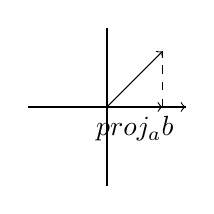
\begin{tikzpicture}
\draw   (1,0) -- (-1, 0)
        (0,1) -- (0,-1);
        \draw[->](0,0) -- (1,0);
        \draw[->](0,0) -- (.7071067,.7071067);
        \draw[->](0,0) -- node[below] {$proj_ab$} ++(.7071067,0);
        \draw[dashed] (.7071067,0) -- (.7071067,.7071067);
\end{tikzpicture}
 $P=\hat{x}a$\hspace{8mm}$\hat{x}=
\frac{
\begin{bmatrix}
1&0\\
\end{bmatrix}
\begin{bmatrix}
cos\theta\\
sin\theta\\
\end{bmatrix}
}
{ 
\begin{bmatrix}
1&0\\
\end{bmatrix}
\begin{bmatrix}
1\\
0\\
\end{bmatrix}
}
= \frac{cos \theta}{1}$ \hspace{8mm}
$
P=
\begin{bmatrix}
cos \theta\\
0\\
\end{bmatrix}
$. \\
(b) 
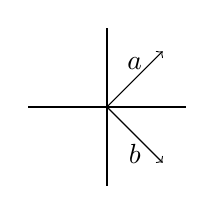
\begin{tikzpicture}
\draw   (1,0) -- (-1, 0)
        (0,1) -- (0,-1);
        \draw[->](0,0) -- node[above] {$a$} ++(.7071067,.7071067);
        \draw[->](0,0) -- node[below] {$b$} ++ (.7071067,-.7071067);
\end{tikzpicture}
 $P=\hat{x}a$\hspace{8mm}$\hat{x}=
\frac{
\begin{bmatrix}
1&-1\\
\end{bmatrix}
\begin{bmatrix}
1\\
1\\
\end{bmatrix}
}
{ 
\begin{bmatrix}
1&1\\
\end{bmatrix}
\begin{bmatrix}
1\\
1\\
\end{bmatrix}
}
= \frac{0}{2}$ \hspace{8mm}
$
P=
\begin{bmatrix}
0\\
0\\
\end{bmatrix}
$. \\
}
\vspace{3mm}
%~~~~~~~~~~~~~~~~~~~~~~~~~~~~~~~~~~~~~~~~~~~~~~~~~~~~~~~~~~~~~~~
\item[4.2.13] (Quick and Recommended) Suppose $A$ is the 4 by 4 identity matrix with its last column removed. $A$ is 4 by 3. Project $b = (1,2,3,4)$ onto the column space of $A$. What shape is the projection matrix $P$ and what is $P$? \\
%~~~~~~~~~~~~~~~~~~~~~ ANSWER TO 4.2.13 ~~~~~~~~~~~~~~~~~~~~~~~~
\vspace{3mm}
\begin{center}
$
A=
\begin{bmatrix}
1&0&0\\
0&1&0\\
0&0&1\\
0&0&0\\
\end{bmatrix}
\rightarrow
P=
\begin{bmatrix}
1&0&0&0\\
0&1&0&0\\
0&0&1&0\\
0&0&0&0\\
\end{bmatrix}
$
 so 
$p=P
\begin{bmatrix}
1\\
2\\
3\\
4\\
\end{bmatrix}
=
\begin{bmatrix}
1\\
2\\
3\\
0\\
\end{bmatrix}
$
\end{center}
\vspace{3mm}
%~~~~~~~~~~~~~~~~~~~~~~~~~~~~~~~~~~~~~~~~~~~~~~~~~~~~~~~~~~~~~~~
\item[4.2.16] What linear combination of (1,2,-1) and (1,0,1) is closest to $b = (2, 1, 1)$? \\
%~~~~~~~~~~~~~~~~~~~~~ ANSWER TO 4.2.16 ~~~~~~~~~~~~~~~~~~~~~~~~
\vspace{3mm}
\begin{center}
$
\begin{bmatrix}
1&1\\
2&0\\
-1&1\\
\end{bmatrix}
\begin{bmatrix}
x_1\\
x_2\\
\end{bmatrix}
=
\begin{bmatrix}
2\\
1\\
1\\
\end{bmatrix}
\hspace{10mm}
P=x_1a_1+x_2a_2
$ \\ \vspace{1mm}
To find $x_1$ and $x_2$ we time both sides of $Ax=b$ by $A^T$. \\ \vspace{1mm}
$
\begin{bmatrix}
1&2&-1\\
1&0&1\\
\end{bmatrix}
\begin{bmatrix}
1&1\\
2&0\\
-1&1\\
\end{bmatrix}
\begin{bmatrix}
x_1\\
x_2\\
\end{bmatrix}
=
\begin{bmatrix}
1&2&-1\\
1&0&1\\
\end{bmatrix}
\begin{bmatrix}
2\\
1\\
1\\
\end{bmatrix}
\rightarrow
\begin{bmatrix}
6&0\\
0&2\\
\end{bmatrix}
\begin{bmatrix}
x_1\\
x_2\\
\end{bmatrix}
=\begin{bmatrix}
3\\
3\\
\end{bmatrix}
\rightarrow
x_1=\frac{1}{2}\hspace{5mm}x_2=\frac{3}{2}
$ \\
$
P=\frac{1}{2}
\begin{bmatrix}
1\\
2\\
-1\\
\end{bmatrix}
+\frac{3}{2}
\begin{bmatrix}
1\\
0\\
1\\
\end{bmatrix}
=
\begin{bmatrix}
2\\
1\\
1\\
\end{bmatrix}
$
\end{center}
\vspace{3mm}
%~~~~~~~~~~~~~~~~~~~~~~~~~~~~~~~~~~~~~~~~~~~~~~~~~~~~~~~~~~~~~~~
\item[4.2.17] (Important) If $P^2 = P$ show that $(I - P)^2 = I - P$. When $P$ projects onto the column space of $A$, $I- P$ projects onto the \underline{\hspace{8mm}}. \\
%~~~~~~~~~~~~~~~~~~~~~ ANSWER TO 4.2.17 ~~~~~~~~~~~~~~~~~~~~~~~~
\vspace{3mm}
\begin{center}
$(I-P)^2=(I-P)(I-P)=I^2-PI-IP+P^2=I-P$ \\
$I-P$ projects onto the left nullspace.
\end{center}
\vspace{3mm}
%~~~~~~~~~~~~~~~~~~~~~~~~~~~~~~~~~~~~~~~~~~~~~~~~~~~~~~~~~~~~~~~
\item[4.2.18] (a) If $P$ is the 2 by 2 projection matrix onto the line through (1,1), then $I - P$ is the projection matrix onto \underline{\hspace{8mm}}. \\
 (b) If $P$ is the 3 by 3 projection matrix onto the line through (1,1,1), then $I - P$ is the projection matrix onto \underline{\hspace{8mm}}. \\
%~~~~~~~~~~~~~~~~~~~~~ ANSWER TO 4.2.18 ~~~~~~~~~~~~~~~~~~~~~~~~
\vspace{3mm}
{\addtolength{\leftskip}{10mm}
(a) $I-P$ projects onto 
$
\begin{bmatrix}
1\\
-1\\
\end{bmatrix}
$ \\
(b) $I-P$ projects onto 
$ \left\{
\begin{bmatrix}
-1\\
0\\
1\\
\end{bmatrix},
\begin{bmatrix}
-1\\
1\\
0\\
\end{bmatrix}
\right\}
$ \\
}
\vspace{3mm}
%~~~~~~~~~~~~~~~~~~~~~~~~~~~~~~~~~~~~~~~~~~~~~~~~~~~~~~~~~~~~~~~
\item[4.2.19] To find the projection matrix onto the plane $x - y - 2z = 0$, choose two vectors in that plane and make them the columns of $A$. The plane should be the column space. Then compute $P = A(A^T A)^{-l} A^T$. \\
%~~~~~~~~~~~~~~~~~~~~~ ANSWER TO 4.2.19 ~~~~~~~~~~~~~~~~~~~~~~~~
\vspace{3mm}
\begin{center}
$
A^T=
\begin{bmatrix}
2&0&1\\
1&1&0\\
\end{bmatrix}
\hspace{15mm}
\begin{bmatrix}
2&1\\
0&1\\
1&0\\
\end{bmatrix}
$ \\
$
A(A^TA)^{-1}A^T=
\begin{bmatrix}
2&1\\
0&1\\
1&0\\
\end{bmatrix}
\left(
\begin{bmatrix}
2&0&1\\
1&1&0\\
\end{bmatrix}
\begin{bmatrix}
2&1\\
0&1\\
1&0\\
\end{bmatrix}
\right)^{-1}
\begin{bmatrix}
2&0&1\\
1&1&0\\
\end{bmatrix}
=
\begin{bmatrix}
5/6&1/6&1/3\\
1/6&5/6&-1/3\\
1/3&-1/3&1/3\\
\end{bmatrix}
$
\end{center}
\vspace{3mm}
%~~~~~~~~~~~~~~~~~~~~~~~~~~~~~~~~~~~~~~~~~~~~~~~~~~~~~~~~~~~~~~~
\item[4.2.26] If an $m$ by $m$ matrix has $A^2 = A$ and its rank is $m$, prove that $A = I$. \\
%~~~~~~~~~~~~~~~~~~~~~ ANSWER TO 4.2.26 ~~~~~~~~~~~~~~~~~~~~~~~~
\vspace{3mm}
\begin{center}
The matrix is a full rank matrix therefore $A^{-1}$ exists. \\
$A^2=A \hspace{3mm} \rightarrow \hspace{3mm} A^{-1}(AA)=A^{-1}A \hspace{3mm} \rightarrow \hspace{3mm} A=I$ \\
\end{center}
\vspace{3mm}
%~~~~~~~~~~~~~~~~~~~~~~~~~~~~~~~~~~~~~~~~~~~~~~~~~~~~~~~~~~~~~~~
\item[4.2.27] The important fact that ends the section is this: If $A^TAx = 0$ then $Ax = 0$. New Proof: The vector $Ax$ is in the nullspace of \underline{\hspace{8mm}}. $Ax$ is always in the column space of \underline{\hspace{8mm}}. To be in both of those perpendicular spaces, $Ax$ must be zero. \\
%~~~~~~~~~~~~~~~~~~~~~ ANSWER TO 4.2.27 ~~~~~~~~~~~~~~~~~~~~~~~~
\vspace{3mm}
{\addtolength{\leftskip}{10mm}
The vector $Ax$ is in the nullspace of \underline{\hspace{3mm}$A^T$\hspace{3mm}}. \\
$Ax$ is always in the column space of \underline{\hspace{3mm}$A$\hspace{3mm}}. \\
So $A$ and $A^TA$ have the same nullspace. \\
}
\vspace{3mm}
%~~~~~~~~~~~~~~~~~~~~~~~~~~~~~~~~~~~~~~~~~~~~~~~~~~~~~~~~~~~~~~~
\item[4.2.29] If $B$ has rank $m$ (full row rank, independent rows) show that $BB^T$ is invertible. \\
%~~~~~~~~~~~~~~~~~~~~~ ANSWER TO 4.2.29 ~~~~~~~~~~~~~~~~~~~~~~~~
\vspace{3mm}
{\addtolength{\leftskip}{10mm}
If $B^T=A$ then $A^TA$ is invertible because $A^TA$ is just a linear combination of independent columns. $A^TA=BB^T$. \\
}
\vspace{3mm}
%~~~~~~~~~~~~~~~~~~~~~~~~~~~~~~~~~~~~~~~~~~~~~~~~~~~~~~~~~~~~~~~
\item[4.2.30] (a) Find the projection matrix $P_c$ onto the column space of $A$ (after looking closely at the matrix!) \\
\begin{center}
$
A=
\begin{bmatrix}
3&6&6\\
4&8&8\\
\end{bmatrix}
$
\end{center}
 (b) Find the 3 by 3 projection matrix $P_R$ onto the row space of $A$. Multiply $B = P_CAP_R$. Your answer $B$ should be a little surprising-can you explain it?  \\
%~~~~~~~~~~~~~~~~~~~~~ ANSWER TO 4.2.30 ~~~~~~~~~~~~~~~~~~~~~~~~
\vspace{3mm}
{\addtolength{\leftskip}{10mm}
(a) 
$
A=
\begin{bmatrix}
3&6&6\\
4&8&8\\
\end{bmatrix}
\hspace{3mm}
A^T=
\begin{bmatrix}
3&4\\
6&8\\
6&8\\
\end{bmatrix}
\hspace{3mm}
C(A)=
\begin{bmatrix}
3\\
4\\
\end{bmatrix}
$ \\
\begin{center}
$
\frac{
\begin{bmatrix}
3\\
4\\
\end{bmatrix}
\begin{bmatrix}
3&4\\
\end{bmatrix}
}{
\begin{bmatrix}
3\\
4\\
\end{bmatrix}
\begin{bmatrix}
3&4\\
\end{bmatrix}
}
=
\frac{1}{25}
\begin{bmatrix}
9&12\\
12&25\\
\end{bmatrix}
$ \\
\end{center}
(b) 
$
C(A^T)=
\begin{bmatrix}
1\\
2\\
2\\
\end{bmatrix}
\hspace{4mm}
P_R=
\frac{
\begin{bmatrix}
1\\
2\\
2\\
\end{bmatrix}
\begin{bmatrix}
1&2&2\\
\end{bmatrix}
}{
\begin{bmatrix}
1\\
2\\
2\\
\end{bmatrix}
\begin{bmatrix}
1&2&2\\
\end{bmatrix}
}
=
\frac{1}{9}
\begin{bmatrix}
1&2&2\\
2&4&4\\
2&4&4\\
\end{bmatrix}
$ \\
\begin{center}
$
B=P_CAP_R=
\begin{bmatrix}
3&6&6\\
4&8&8\\
\end{bmatrix}
$ \\ \vspace{1mm}
This is because the columns of $A$ projected onto themselves will just be $A$ and by similar logic $AP_R$ will just be $A$ as well. Therefore $P_CAP_R=A$. \\
\end{center}
}
\vspace{3mm}
%~~~~~~~~~~~~~~~~~~~~~~~~~~~~~~~~~~~~~~~~~~~~~~~~~~~~~~~~~~~~~~~

\end{enumerate}
\vspace{5mm}
\textbf{Chapter 4.3}
\begin{enumerate}
\item[4.3.6] Project $\pmb{b} = (0, 8, 8, 20)$ onto the line through $\pmb{a} = (1, 1, 1, 1)$. Find $\hat{x} = \pmb{a}^T\pmb{b}/\pmb{a}^T\pmb{a}$ and the projection $\pmb{p} = \hat{x}\pmb{a}$. Check that $\pmb{e} = \pmb{b} - \pmb{p}$ is perpendicular to $\pmb{a}$, and find the shortest distance $\lVert\pmb{e}\rVert$ from $\pmb{b}$ to the line through $\pmb{a}$\\
%~~~~~~~~~~~~~~~~~~~~~ ANSWER TO 4.3.6 ~~~~~~~~~~~~~~~~~~~~~~~~
\vspace{3mm}
$
$$
a =
\begin{bmatrix}
1\\
1\\
1\\
1\\
\end{bmatrix}
\hspace{3mm}
\begin{bmatrix}
0\\
8\\
8\\
20\\
\end{bmatrix}
$$
$\\
$\hat{x} = \frac{a^Tb}{a^Ta} =$
$
$$
\frac{
\begin{bmatrix}
1&1&1&1
\end{bmatrix}
\begin{bmatrix}
0\\
8\\
8\\
20\\
\end{bmatrix}
}{
\begin{bmatrix}
1&1&1&1
\end{bmatrix}
\begin{bmatrix}
1\\
1\\
1\\
1\\
\end{bmatrix}
}
= \frac{36}{4} = 9 \hspace{3mm} p = \hat{x}a =
\begin{bmatrix}
9\\
9\\
9\\
9\\
\end{bmatrix}
$$
$\\
$
$$
b - p = e
\begin{bmatrix}
0\\
8\\
8\\
20\\
\end{bmatrix}
-
\begin{bmatrix}
-9\\
-1\\
-1\\
11\\
\end{bmatrix}
\pmb{\cdot}
\begin{bmatrix}
1\\
1\\
1\\
1\\
\end{bmatrix}
= 0 \hspace{1mm}\checkmark
$$
$\\
$\lVert e \rVert = \sqrt{204}$\\

\vspace{3mm}
%~~~~~~~~~~~~~~~~~~~~~~~~~~~~~~~~~~~~~~~~~~~~~~~~~~~~~~~~~~~~~~~
\item[4.3.9] For the closest parabola $b = C + Dt + Et^2$ to the same four points, write down the unsolvable equations $Ax = b$ in three unknowns $x = (C, D, E)$. Set up the three normal equations $A^TA\hat{x} = A^Tb$ (solution not required). In Figure 4.9a you are now fitting a parabola to 4 points - what is happening in Figure 4.9b?\\
%~~~~~~~~~~~~~~~~~~~~~ ANSWER TO 4.3.9 ~~~~~~~~~~~~~~~~~~~~~~~~
\vspace{3mm}
$
$$
\begin{bmatrix}
1&0&0\\
1&1&1\\
1&3&9\\
1&4&16\\
\end{bmatrix}
\begin{bmatrix}
C\\
D\\
E\\
\end{bmatrix}
=
\begin{bmatrix}
0\\
8\\
8\\
20\\
\end{bmatrix}
\rightarrow
\begin{bmatrix}
1&1&1&1\\
0&1&3&4\\
0&1&9&16\\
\end{bmatrix}
\begin{bmatrix}
1&0&0\\
1&1&1\\
1&3&9\\
1&4&16\\
\end{bmatrix}
\begin{bmatrix}
C\\
D\\
E\\
\end{bmatrix}
=
\begin{bmatrix}
1&1&1&1\\
0&1&3&4\\
0&1&9&16\\
\end{bmatrix}
\begin{bmatrix}
0\\
8\\
8\\
20\\
\end{bmatrix}
\rightarrow
$$
$\\
\vspace{3mm}
$
$$
\begin{bmatrix}
4&8&26\\
8&26&92\\
26&92&338\\
\end{bmatrix}
\begin{bmatrix}
C&D&E
\end{bmatrix}
=
\begin{bmatrix}
36\\
112\\
400\\
\end{bmatrix}
$$
$\\
\vspace{6mm}
%~~~~~~~~~~~~~~~~~~~~~~~~~~~~~~~~~~~~~~~~~~~~~~~~~~~~~~~~~~~~~~~
\item[4.3.12] (Recommended) This problem projects $\pmb{b} = (b_1, ...,b_m)$ onto the line through $a = (1,...,1)$. We solve $m$ equations $ax = b$ in 1 unknown (by least squares).\\
(a) Solve $a^Ta\hat{x} = a^Tb$ to show that $\hat{x}$ is the \textit{mean} (the average) of the $b$'s.\\
%~~~~~~~~~~~~~~~~~~~~~ ANSWER TO 4.3.12 ~~~~~~~~~~~~~~~~~~~~~~~~
\vspace{3mm}
$
$$
\begin{bmatrix}
11\cdots11\\
\end{bmatrix}
\begin{bmatrix}
1\\
1\\
\cdot\\
\cdot\\
\cdot\\
1\\
1\\
\end{bmatrix}
\hat{x}
=
\begin{bmatrix}
11\cdots11\\
\end{bmatrix}
\begin{bmatrix}
b_1\\
\cdot\\
\cdot\\
\cdot\\
b_m
\end{bmatrix}
$$
$\\
$=$ (number of components in a) $\hat{x} = \sum_{i = 1}^{m}b_i \rightarrow\frac{ \hat{x} = \sum_{i = 1}^{m}b_i}{number \hspace{1mm}of\hspace{1mm} components} =$ average\\
\vspace{3mm}
%~~~~~~~~~~~~~~~~~~~~~~~~~~~~~~~~~~~~~~~~~~~~~~~~~~~~~~~~~~~~~~~
(b) Find $e = b - a\hat{x}$ and the \textit{variance} $\lVert e \rVert^2$ and the \textit{standard deviation} $\lVert e \rVert$.\\
%~~~~~~~~~~~~~~~~~~~~~ ANSWER TO 4.3.12 ~~~~~~~~~~~~~~~~~~~~~~~~
\vspace{3mm}
$
$$
e =
\begin{bmatrix}
b_1\\
\cdot\\
\cdot\\
\cdot\\
b_m
\end{bmatrix}
-
\begin{bmatrix}
\hat{x}\\
\cdot\\
\cdot\\
\cdot\\
\hat{x}\\
\end{bmatrix}
=
\begin{bmatrix}
b_1 - \hat{x}\\
\cdot\\
\cdot\\
\cdot\\
b_m - \hat{x}\\
\end{bmatrix}
$$
$\\
\vspace{3mm}
$
$$
\lVert e \rVert^2 = \sum_{i = 1}^m(b_i - \hat{x})^2 =
$$
$
variance\\
\vspace{3mm}
%~~~~~~~~~~~~~~~~~~~~~~~~~~~~~~~~~~~~~~~~~~~~~~~~~~~~~~~~~~~~~~~
(c) The horizontal line $\hat{b} = 3$ is closest to $b = (1, 2, 6)$. Check that $p = (3, 3, 3)$ is perpendicular to $e$ \\
\hspace{6mm}and find the 3 by 3 projection matrix $P$.\\
%~~~~~~~~~~~~~~~~~~~~~ ANSWER TO 4.3.12 ~~~~~~~~~~~~~~~~~~~~~~~~
\vspace{3mm}
$
$$
e = b - p =
\begin{bmatrix}
1\\
2\\
6\\
\end{bmatrix}
-
\begin{bmatrix}
3\\
3\\
3\\
\end{bmatrix}
=
\begin{bmatrix}
-2\\
-1\\
3\\
\end{bmatrix}
\pmb{\cdot}
\begin{bmatrix}
3\\
3\\
3\\
\end{bmatrix}
= -6-3+9 = 0 \hspace{2mm}\checkmark
$$
$\\
\vspace{3mm}
$
$$
P = 
\frac{1}{3}
\begin{bmatrix}
1&1&1\\
1&1&1\\
1&1&1\\
\end{bmatrix}
$$
$
\vspace{3mm}
%~~~~~~~~~~~~~~~~~~~~~~~~~~~~~~~~~~~~~~~~~~~~~~~~~~~~~~~~~~~~~~~
\item[4.3.22] Find the best line $C + Dt$ to fit $b = 4, 2, -1, 0, 0$ at times $t = -2, -1, 0, 1, 2$.\\
%~~~~~~~~~~~~~~~~~~~~~ ANSWER TO 4.3.22 ~~~~~~~~~~~~~~~~~~~~~~~~
\vspace{3mm}
$
$$
\begin{bmatrix}
1&-2\\
1&-1\\
1&0\\
1&1\\
1&2\\
\end{bmatrix}
\begin{bmatrix}
C\\
D\\
\end{bmatrix}
=
\begin{bmatrix}
4\\
2\\
-1\\
0\\
0\\
\end{bmatrix}
\rightarrow
\begin{bmatrix}
1&1&1&1&1\\
-2&-1&0&1&2\\
\end{bmatrix}
\begin{bmatrix}
1&-2\\
1&-1\\
1&0\\
1&1\\
1&2\\
\end{bmatrix}
\begin{bmatrix}
C\\
D\\
\end{bmatrix}
=
\begin{bmatrix}
1&1&1&1&1\\
-2&-1&0&1&2\\
\end{bmatrix}
\begin{bmatrix}
4\\
2\\
-1\\
0\\
0\\
\end{bmatrix}
\rightarrow
$$
$\\
\vspace{3mm}
$
$$
\begin{bmatrix}
5&0\\
0&10\\
\end{bmatrix}
\begin{bmatrix}
C\\
D\\
\end{bmatrix}
=
\begin{bmatrix}
5\\
-10\\
\end{bmatrix}
\hspace{3mm} C = 1 \hspace{3mm} D = -1
$$
$\\
\vspace{3mm}
%~~~~~~~~~~~~~~~~~~~~~~~~~~~~~~~~~~~~~~~~~~~~~~~~~~~~~~~~~~~~~~~
\item[4.3.26] Find the \textit{plane} that gives the best fit to the 4 values $b = (0, 1, 3, 4)$ at the corners $(1, 0)$ and $(0, 1)$ and $(-1, 0) and (0, -1)$ of a square. The equations $C + Dx + Ey = b$ at those 4 points are $Ax = b$ with 3 unknowns $x = (C, D, E)$. What is $A$? At the center $(0, 0)$ of the square, show that $C + Dx + Ey =$ average of the $b$'s.\\
%~~~~~~~~~~~~~~~~~~~~~ ANSWER TO 4.3.26 ~~~~~~~~~~~~~~~~~~~~~~~~
\vspace{3mm}
$
$$
\begin{bmatrix}
1&1&0\\
1&0&1\\
1&-1&0\\
1&0&-1\\
\end{bmatrix}
\begin{bmatrix}
C\\
D\\
E\\
\end{bmatrix}
=
\begin{bmatrix}
0\\
1\\
3\\
4\\
\end{bmatrix}
\rightarrow
\begin{bmatrix}
1&1&1&1\\
1&0&-1&0\\
0&1&0&-1\\
\end{bmatrix}
\begin{bmatrix}
1&1&0\\
1&0&1\\
1&-1&0\\
1&0&-1\\
\end{bmatrix}
\begin{bmatrix}
C\\
D\\
E\\
\end{bmatrix}
=
\begin{bmatrix}
1&1&1&1\\
1&0&-1&-\\
0&1&0&-1\\
\end{bmatrix}
\begin{bmatrix}
0\\
1\\
3\\
4\\
\end{bmatrix}
$$
$\\
$
$$
\begin{bmatrix}
4&0&0\\
0&2&0\\
0&0&2\\
\end{bmatrix}
\begin{bmatrix}
C\\
D\\
E\\
\end{bmatrix}
=
\begin{bmatrix}
8\\
-3\\
-3\\
\end{bmatrix}
\hspace{3mm} C = 2 \hspace{3mm} D = \frac{-3}{2} = E
$$
$\\
$p = 2 - \frac{3}{2}x - \frac{3}{2}y$\\
at $x = y = 0 \hspace{3mm} p = 2$, which is the average of the square\\
\vspace{3mm}
%~~~~~~~~~~~~~~~~~~~~~~~~~~~~~~~~~~~~~~~~~~~~~~~~~~~~~~~~~~~~~~~

\end{enumerate}
\vspace{5mm}
\textbf{Chapter 4.4}
\begin{enumerate}
\item[4.4.1] Are these pairs of vectors orthonormal or only orthogonal or only independent?\\
\vspace{2mm}
(a) $\left[\begin{smallmatrix} 1\\ 0 \end{smallmatrix} \right]$ and $\left[\begin{smallmatrix} -1\\ 1 \end{smallmatrix} \right]$ \hspace{3mm} (b) $\left[\begin{smallmatrix} .6\\ .8 \end{smallmatrix} \right]$ and $\left[\begin{smallmatrix} .4\\ -.3 \end{smallmatrix} \right]$ \hspace{3mm} (c) $\left[\begin{smallmatrix} cos\theta\\ sin\theta \end{smallmatrix} \right]$ and $\left[\begin{smallmatrix} -sin\theta\\ cos\theta \end{smallmatrix} \right]$.\\
\vspace{2mm}
Change the second vector when necessary to produce orthonormal vectors.\\
%~~~~~~~~~~~~~~~~~~~~~ ANSWER TO 4.4.1 ~~~~~~~~~~~~~~~~~~~~~~~~
\vspace{3mm}
(a) independent, the second vector would be $\left[\begin{smallmatrix} 0\\ 1 \end{smallmatrix} \right]$ to be orthonormal\\
\vspace{3mm}
(b) orthogonal, the second vector would be $\left[\begin{smallmatrix} .8\\ -.6\end{smallmatrix} \right]$ to be orthonoraml and independent\\
\vspace{3mm}
(c) orthonormal and independent\\
\vspace{3mm}

%~~~~~~~~~~~~~~~~~~~~~~~~~~~~~~~~~~~~~~~~~~~~~~~~~~~~~~~~~~~~~~~
\item[4.4.4] Give an example of each of the following:\\
(a) A matrix $Q$ that has orthonormal columns but $QQ^T \neq I$.\\
\vspace{3mm}
$
$$
Q =
\begin{bmatrix}
2&1\\
2&-1\\
\end{bmatrix}
QQT=
\begin{bmatrix}
2&1\\
2&-1\\
\end{bmatrix}
\begin{bmatrix}
2&2\\
1&-1\\
\end{bmatrix}
=
\begin{bmatrix}
5&3\\
3&5\\
\end{bmatrix}
\neq I
$$
$\\
\vspace{3mm}
(b) Two orthogonal vectors that are not linearly independent.\\
\vspace{3mm}
$
$$
\begin{bmatrix}
0\\
1\\
\end{bmatrix}
\begin{bmatrix}
0\\
0\\
\end{bmatrix}
$$
$\\
\vspace{3mm}
(c) An orthonormal basis for $\pmb{R}^3$, including the vector $q_1 = (1, 1, 1)/\sqrt{3}$.\\
%~~~~~~~~~~~~~~~~~~~~~ ANSWER TO 4.4.4 ~~~~~~~~~~~~~~~~~~~~~~~~
\vspace{3mm}
$
$$
\begin{bmatrix}
\frac{1}{\sqrt{3}}\\
\frac{1}{\sqrt{3}}\\
\frac{1}{\sqrt{3}}\\
\end{bmatrix}
,
\begin{bmatrix}
1\\
-1\\
0\\
\end{bmatrix}
,
\begin{bmatrix}
1\\
0\\
-1\\
\end{bmatrix}
$$
$
\vspace{3mm}
%~~~~~~~~~~~~~~~~~~~~~~~~~~~~~~~~~~~~~~~~~~~~~~~~~~~~~~~~~~~~~~~
\item[4.4.10] Orthonormal vectors are automatically linearly independent.\\
(a) Vector proof: When $c_1q_1 + c_2+q_2 + c_3q_3 = 0$, what dot product leads to $c_1 = 0$? Similarly $c_2 = 0$ and $c_3 = 0$. Thus the $q$'s are independent.\\
\vspace{3mm}
If all the q's are orthonormal then the dot product of $q_1$ with $c_1q_1 + c_2q_2 + c_3q_3 = 0$ gives $c_1 = 0$. Similarly $c_2 = c_3 = 0$.\\ 
\vspace{3mm}
(b) Matrix proof: Show that $Qx = 0$ leads to $x = 0$. Since $Q$ may be rectangular, you can use $Q^T$ but not $Q^{-1}$.\\
%~~~~~~~~~~~~~~~~~~~~~ ANSWER TO 4.4.10 ~~~~~~~~~~~~~~~~~~~~~~~~
\vspace{3mm}
$Qx = 0 \rightarrow Q^TQx = 0 \rightarrow x = 0$\\
\vspace{3mm}
%~~~~~~~~~~~~~~~~~~~~~~~~~~~~~~~~~~~~~~~~~~~~~~~~~~~~~~~~~~~~~~~
\item[4.4.11] (a) Gram-Shmidt: Find orthonormal vectors $q_1$ and $q_2$ in the plane spanned by $a = (1, 3, 4, 5, 7)$ and\\
\hspace{6mm}$b = (-6, 6, 8, 0, 8)$.\\
\vspace{3mm}
$\frac{1}{10}(1, 3, 4, 5, 7) \hspace{3mm} \frac{1}{10}(-7, 3, 4, -5, 1)$\\
\vspace{3mm}
(b) Which vector in this plane is closest to $(1, 0, 0, 0, 0)$?\\
%~~~~~~~~~~~~~~~~~~~~~ ANSWER TO 4.4.11 ~~~~~~~~~~~~~~~~~~~~~~~~
\vspace{3mm}
$
$$
\frac{1}{10}
\begin{bmatrix}
1&-7\\
3&3\\
4&4\\
5&-5\\
7&1\\
\end{bmatrix}
\frac{1}{10}
\begin{bmatrix}
1&3&4&5&7\\
-7&3&4&-5&1\\
\end{bmatrix}
= 
\frac{1}{100}
\begin{bmatrix}
50&-18&-24&40&0\\
-18&18&24&0&24\\
-24&24&32&0&32\\
40&0&0&50&30\\
0&24&32&30&50\\
\end{bmatrix}
\begin{bmatrix}
1\\
0\\
0\\
0\\
0\\
\end{bmatrix}
=
\frac{1}{100}
\begin{bmatrix}
50\\
-18\\
-24\\
40\\
0\\
\end{bmatrix}
=
\begin{bmatrix}
.5\\
-.18\\
-.24\\
.4\\
0\\
\end{bmatrix}
$$
$\\
\vspace{40mm}
%~~~~~~~~~~~~~~~~~~~~~~~~~~~~~~~~~~~~~~~~~~~~~~~~~~~~~~~~~~~~~~~
\item[4.4.15] (a) Find orthonormal vectors $q_1, q_2, q_3$ such that $q_1$, $q_2$ span the column space of\\
\begin{center}
$
$$
A =
\begin{bmatrix}
1&1\\
2&-1\\
-2&4\\
\end{bmatrix}
$$
$\\
\vspace{3mm}
$q_1 = \frac{1}{3} (1, 2, -2) \hspace{3mm} q_2 = \frac{1}{3}(2, 1, 2) \hspace{3mm} q_3 = \frac{1}{3}(2, 2, -1)$\\
\vspace{3mm}
\end{center}
(b) Which of the four fundamental subspaces contains $q_3$?\\
\vspace{3mm}
the left nullspace\\
\vspace{3mm}
(c) Solve $Ax = (1, 2, 7)$ by least squares.\\
%~~~~~~~~~~~~~~~~~~~~~ ANSWER TO 4.4.15 ~~~~~~~~~~~~~~~~~~~~~~~~
\vspace{3mm}
$\hat{x} = (A^TA)^{-1}A^T$
$
$$
\begin{bmatrix}
1\\
2\\
7\\
\end{bmatrix}
=
\left(
\begin{bmatrix}
1&2&-2\\
1&-1&4\\
\end{bmatrix}
\begin{bmatrix}
1&1\\
2&-1\\
-2&4\\
\end{bmatrix}
\right)
\begin{bmatrix}
1&2&-2\\
1&-1&4\\
\end{bmatrix}
\begin{bmatrix}
1\\
2\\
7\\
\end{bmatrix}
\rightarrow
\begin{bmatrix}
9&-9\\
-9&18\\
\end{bmatrix}
^{-1}
\begin{bmatrix}
-9\\
27\\
\end{bmatrix}
=
\frac{1}{9}
\begin{bmatrix}
2&1\\
1&1\\
\end{bmatrix}
\begin{bmatrix}
-9\\
27\\
\end{bmatrix}
=
\frac{1}{9}
\begin{bmatrix}
9\\
18\\
\end{bmatrix}
=
\begin{bmatrix}
1\\
2\\
\end{bmatrix}
$$
$
\vspace{3mm}
%~~~~~~~~~~~~~~~~~~~~~~~~~~~~~~~~~~~~~~~~~~~~~~~~~~~~~~~~~~~~~~~
\item[4.4.23] Find $q_1, q_2, q_3$ (orthonormal) as combinations of $a, b, c$ (independent columns). Then write $A$ as $QR$:\\
\begin{center}
$
$$
c =
\begin{bmatrix}
1&2&4\\
0&0&5\\
0&3&6\\
\end{bmatrix}
$$
$.\\
\end{center}
%~~~~~~~~~~~~~~~~~~~~~ ANSWER TO 4.4.23 ~~~~~~~~~~~~~~~~~~~~~~~~
\vspace{3mm}
A is an invertible matrix so the vectors $q_1 = \left[\begin{smallmatrix} 1\\ 0\\ 0 \end{smallmatrix}\right]$, $q_2 = \left[\begin{smallmatrix} 0\\ 1\\ 0 \end{smallmatrix}\right]$, $q_3 = \left[\begin{smallmatrix} 0\\ 0\\ 1 \end{smallmatrix}\right]$ in the column space and are orthonormal.\\
\vspace{3mm}
$
$$
A =
\begin{bmatrix}
1&0&0\\
0&1&0\\
0&0&1\\
\end{bmatrix}
\begin{bmatrix}
1&2&4\\
0&0&5\\
0&3&6\\
\end{bmatrix}
$$
$
\vspace{3mm}
%~~~~~~~~~~~~~~~~~~~~~~~~~~~~~~~~~~~~~~~~~~~~~~~~~~~~~~~~~~~~~~~
\item[4.4.24] (a) Find a basis for the subspace $S$ in $R^4$ spanned by all solutions of\\
\begin{center}
$x_1 + x_2 + x_3 - x_4 = 0$\\
\vspace{3mm}
$
$$
S = 
\left\{
\begin{bmatrix}
1\\
0\\
0\\
1\\
\end{bmatrix}
,
\begin{bmatrix}
1\\
-1\\
0\\
0\\
\end{bmatrix}
,
\begin{bmatrix}
1\\
0\\
-1\\
0\\
\end{bmatrix}
\right\}
$$
$
\end{center}
(b) Find a basis for the orthogonal comblement $S^{\perp}$.\\
\vspace{3mm}
Since all vectors and all their linear combinations contained in S are orthogonal to the orginal matrix $\left[\begin{smallmatrix} 1\\ 1\\ 1\\ -1 \end{smallmatrix}\right], S\perp$ is the original matrix $\left[\begin{smallmatrix}1\\ 1\\ 1\\ -1\end{smallmatrix}\right]$\\
\vspace{3mm}
(c) Find $b_1$ in $S$ and $b_2$ in $S^{\perp}$ so that $b_1 + b_2 = b = (1, 1, 1, 1)$.\\
%~~~~~~~~~~~~~~~~~~~~~ ANSWER TO 4.4.24 ~~~~~~~~~~~~~~~~~~~~~~~~
\vspace{3mm}

%~~~~~~~~~~~~~~~~~~~~~~~~~~~~~~~~~~~~~~~~~~~~~~~~~~~~~~~~~~~~~~~
\item[4.4.34] $Q = I - 2uu^T$ is a reflection matrix when $u^Tu = 1$. Two reflections give $Q^2 = I$.\\
(a) Show that $Qu = -u$. The mirror is perpendicular to $u$.\\
\vspace{3mm}
$Q = I - 2uu^T \rightarrow Qu = Iu - 2uu^Tu$ Since $u^Tu = 1 \rightarrow Qu = -u$\\
\vspace{3mm}
(b) Find $Qv$ when $u^Tv = 0$. The mirror contains $v$. It reflects to itself.\\
%~~~~~~~~~~~~~~~~~~~~~ ANSWER TO 4.4.34 ~~~~~~~~~~~~~~~~~~~~~~~~
\vspace{3mm}
$Q = I - 2uu^T \rightarrow Qv = Iv - 2uu^Tv$ since $u^Tv = 0 \rightarrow Qv = v$
\vspace{3mm}
%~~~~~~~~~~~~~~~~~~~~~~~~~~~~~~~~~~~~~~~~~~~~~~~~~~~~~~~~~~~~~~~
\end{enumerate}
\end{document}  